%----------
% Formato:
%----------

\documentclass[a4paper,12pt,spanish,final]{epsc_tfc_pfc}
\usepackage[spanish,english]{babel}
\usepackage[latin1]{inputenc}
\usepackage{amssymb,amsmath, amsfonts}
\usepackage{array}
\begin{document}
\pagestyle{empty}
\selectlanguage{spanish}
\portada

%----------
% Resumen:
%----------

\begin{resum}{16cm}
Aquesx document cont� les pautes del format de presentaci� del treball o projecte de final de carrera. En tot cas, cal tenir en compte el que estableix la ``Normativa del treball de fi de carrera (TFC) i del projecte de fi de carrera (PFC)'' aprovada per la Comissi� Permanent de l'EPSC, especialment l'apartat ``Requeriments del treball''.
\end{resum}
\selectlanguage{english}
\begin{overview}{15cm}
This document contains guidelines for writing your TFC/PFC\@. However, you should also take into consideration the standards established in the document Normativa del treball de fi de carrera (TFC) i del projecte de fi de carrera (PFC), paying special attention to the section Requeriments del treball, as this document has been approved by the EPSC Standing Committee
\end{overview}
\selectlanguage{spanish}

%--------------
% Dedicatoria:
%--------------

\begin{dedicatoria}
Escriure aqu� opcionalment la dedicat�ria.
\end{dedicatoria}

%-------------------
% Figuras y tablas:
%-------------------

\thispagestyle{empty}
\tableofcontents
\cleardoublepage
\thispagestyle{empty}
\listoffigures
\cleardoublepage
\thispagestyle{empty}
\listoftables
\cleardoublepage
\pagestyle{fancy}

%---------------
% Introducci�n:
%---------------

\begin{intro}{Introducci�n}

En el contexto de este trabajo entendemos por \emph{aprovisionamiento de un sistema} al conjunto de acciones que se deben realizar para disponer de un equipo, ya sea f�sico o virtual, con un m�nimo sistema operativo instanciado y accesible a nivel TCP/IP\@. En el caso de los sistemas f�sicos, no consideramos las tareas de desempaquetado, ensamblaje, enracado y cableado de los hierros porque se deben realizar en cada centro de datos por un equipo local de operaciones.

Aprovisionar un sistema de forma manual puede suponer entre 20 y 30 minutos. La mayor parte del tiempo se invierte esperando y respondiendo al asistente de instalaci�n. Para ello, adem�s, es necesario tener acceso a la entrada y salida estandar del equipo para visualizar e interactuar con el asistente. T�picamente, con un teclado y un monitor o una redirecci�n de los mismos mediante protocolos tipo \emph{Remote Frame Buffer} o \emph{X Window System Core Protocol}.

Aprovisionar de forma manual es un requisito previo a la automatizaci�n ya que nos ayuda a entender las dependencias de orden y a identificar las acciones b�sicas que se deben realiza para conseguir un sistema funcional. Existe, sin embargo, un elemento mucho mas dif�cil de reemplazar, capaz de explorar el entorno, identificar casu�sticas y en definitiva tomar decisiones. El cerebro humano.

No se trata de dar mucha inteligencia al sistema de aprovisionamiento sin� de consensar un modelo sencillo y predictible que resulte eficaz en su funcionamiento y simple de mantener. A lo largo de la etapa de aprovisionado intervienen distintas tecnolog�as que se complementan entre s�: PXE, DHCP, TFTP, DNS, Kickstart, YUM, KOAN, Libvirt y KVM\@. La soluci�n propuesta, utiliza una herramienta de c�digo abierto llamada \emph{Cobbler} que combina y centraliza la gesti�n de muchas de las tecnolog�as mencionadas.

Una vez aprovisionados, los sistemas sirven de base sobre la que podemos desplegar servicios. Los servicios determinan el rol o la raz�n de ser de cada equipo. Si bien en la fase de aprovisionado este rol se perfila sutilmente, no es hasta la fase de despliegue, donde se definen con exactitud las funciones de cada equipo y las interrelaciones entre los mismos.

A vista de p�jaro el sistema est� compuesto por dos grandes bloques funcionales que aglutinan varios servicios; el primer bloque, representado por Cobbler, se encarga de todas las funciones relacionadas con el aprovisionamiento de sistemas. El segundo bloque, representado por Puppet, se encarga de desplegar los servicios y de mantenerlos en el estado deseado.

\begin{figure}[t]
  \centering
    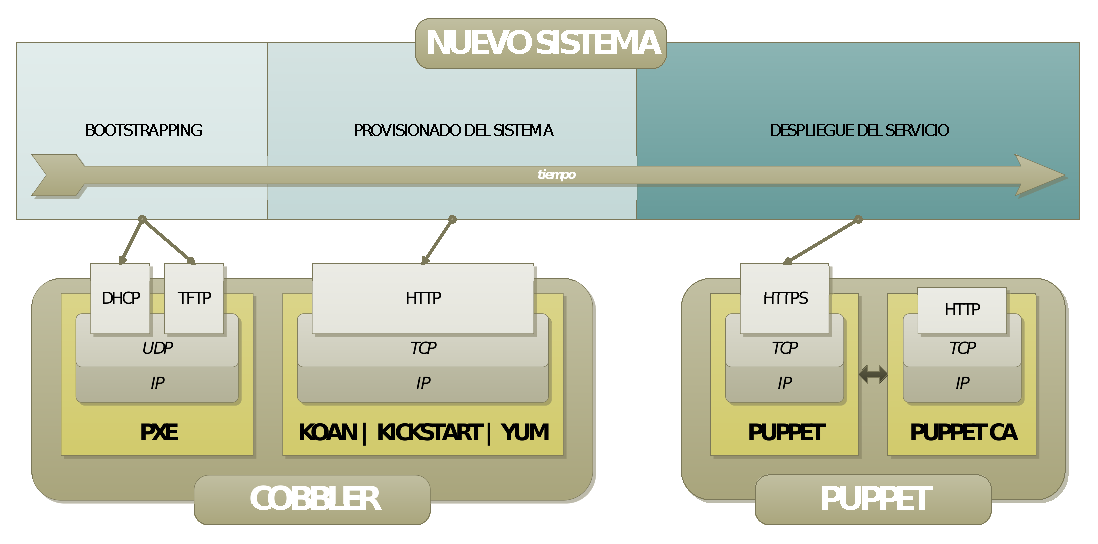
\includegraphics[scale=0.83]{intro}
  \caption{A vista de p�jaro.}
\end{figure}

Blah blah blah blah blah blah blah blah blah blah blah blah blah blah blah blah blah blah blah blah blah blah blah blah blah blah blah blah blah blah blah blah blah blah blah blah blah blah blah blah blah blah blah blah blah blah blah blah blah blah blah blah blah blah blah blah blah blah blah blah blah blah blah blah blah blah blah blah blah blah blah blah blah blah blah blah blah blah blah blah blah blah blah blah blah blah blah blah blah blah blah blah blah blah blah blah blah blah blah blah blah blah blah.

Blah blah blah blah blah blah blah blah blah blah blah blah blah blah blah blah blah blah blah blah blah blah blah blah blah blah blah blah blah blah blah blah blah blah blah blah blah blah blah blah blah blah blah blah blah blah blah blah blah blah blah blah blah blah blah blah blah blah blah blah blah blah blah blah blah blah blah blah blah blah blah blah blah blah blah blah blah blah blah blah blah blah blah blah blah blah blah blah blah blah blah blah blah blah blah blah blah blah blah blah blah blah blah.

Blah blah blah blah blah blah blah blah blah blah blah blah blah blah blah blah blah blah blah blah blah blah blah blah blah blah blah blah blah blah blah blah blah blah blah blah blah blah blah blah blah blah blah blah blah blah blah blah blah blah blah blah blah blah blah blah blah blah blah blah blah blah blah blah blah blah blah blah blah blah blah blah blah blah blah blah blah blah blah blah blah blah blah blah blah blah blah blah blah blah blah blah blah blah blah blah blah blah blah blah blah blah blah.
\end{intro}

\pagestyle{fancy}

%----------
% Cobbler:
%----------

\chapter{Cobbler}
Cobbler is a Linux installation server that allows for rapid setup of network installation environments. It glues together and automates many associated Linux tasks so you do not have to hop between lots of various commands and applications when rolling out new systems, and, in some cases, changing existing ones. It can help with installation, DNS, DHCP, package updates, power management, configuration management orchestration, and much more.
\section{Tecnolog�as}
\subsection{PXE: Preboot eXecution Environment}
\subsection{Kickstart}
\subsection{YUM: Yellowdog Updater Modified}
\subsection{KOAN: Kickstart Over A Network}
\section{Aprovisionado}
\subsection{F�sico}
\subsection{Virtual}

%---------
% Puppet:
%---------

\chapter{Puppet}
\section{Tecnolog�as}
\subsection{DSL: Domain Specific Language}
\subsection{Cliente - Servidor}
\subsection{Framework}
\section{Despliegue}

%---------------
% Bibliografia:
%---------------

\begin{thebibliography}{2}

%% Llibres:  Autor/s (cognoms i inicials dels noms), t�tol del llibre (en cursiva), editor, ciutat i any de publicaci�. Quan es cita el cap�tol d'un llibre s'ha d'indicar el t�tol del cap�tol (entre cometes), el t�tol del llibre (en cursiva) i els n�meros de p�gines amb la primera i la darrera incloses.

%%  Exemple de capitol en llibre
\bibitem{prova1}
Cognoms-autor, Inicial-nom.
``T�tol del cap�tol''. {\it T�tol del llibre}.
(Editor. Ciutat. Any publicaci�): pagina1--paginaN.

%%  Exemple de d'article en revista
\bibitem{prova2}
Cognoms-autor, Inicial-nom.
``T�tol de l'article''. {\it T�tol de la revista}.
{\bf volum}(numero),
pagina1--paginaN. (Any publicaci�)

\end{thebibliography}
\end{document}
